\documentclass[12pt,a4paper]{article}
\usepackage[T2A]{fontenc}
\usepackage[utf8]{inputenc}
\usepackage[russian]{babel}
\usepackage[a4paper,margin=2cm]{geometry}
\usepackage{graphicx}
\usepackage{caption}
\usepackage{hyperref}
\usepackage{longtable}
\usepackage{array}
\usepackage{booktabs}
\usepackage{float}
\usepackage{listings}
\captionsetup{justification=centering,font=small}
\lstset{
  basicstyle=\ttfamily\footnotesize,
  breaklines=true,
  columns=fullflexible,
  keepspaces=true,
  frame=single,
  tabsize=2,
  literate={а}{{\cyra}}1{б}{{\cyrb}}1{в}{{\cyrv}}1{г}{{\cyrg}}1{д}{{\cyrd}}1
           {е}{{\cyre}}1{ё}{{\"e}}1{ж}{{\cyrzh}}1{з}{{\cyrz}}1{и}{{\cyri}}1
           {й}{{\cyrishrt}}1{к}{{\cyrk}}1{л}{{\cyrl}}1{м}{{\cyrm}}1{н}{{\cyrn}}1
           {о}{{\cyro}}1{п}{{\cyrp}}1{р}{{\cyrr}}1{с}{{\cyrs}}1{т}{{\cyrt}}1
           {у}{{\cyru}}1{ф}{{\cyrf}}1{х}{{\cyrh}}1{ц}{{\cyrc}}1{ч}{{\cyrch}}1
           {ш}{{\cyrsh}}1{щ}{{\cyrshch}}1{ъ}{{\cyrhrdsn}}1{ы}{{\cyrery}}1
           {ь}{{\cyrsftsn}}1{э}{{\cyrerev}}1{ю}{{\cyryu}}1{я}{{\cyrya}}1
           {А}{{\CYRA}}1{Б}{{\CYRB}}1{В}{{\CYRV}}1{Г}{{\CYRG}}1{Д}{{\CYRD}}1
           {Е}{{\CYRE}}1{Ё}{{\"E}}1{Ж}{{\CYRZH}}1{З}{{\CYRZ}}1{И}{{\CYRI}}1
           {Й}{{\CYRISHRT}}1{К}{{\CYRK}}1{Л}{{\CYRL}}1{М}{{\CYRM}}1{Н}{{\CYRN}}1
           {О}{{\CYRO}}1{П}{{\CYRP}}1{Р}{{\CYRR}}1{С}{{\CYRS}}1{Т}{{\CYRT}}1
           {У}{{\CYRU}}1{Ф}{{\CYRF}}1{Х}{{\CYRH}}1{Ц}{{\CYRC}}1{Ч}{{\CYRCH}}1
           {Ш}{{\CYRSH}}1{Щ}{{\CYRSHCH}}1{Ъ}{{\CYRHRDSN}}1{Ы}{{\CYRERY}}1
           {Ь}{{\CYRSFTSN}}1{Э}{{\CYREREV}}1{Ю}{{\CYRYU}}1{Я}{{\CYRYA}}1
}
\hypersetup{colorlinks=true,linkcolor=black,urlcolor=blue}
\begin{document}
\begin{titlepage}
  \centering
  \vspace*{1cm}
  {\LARGE \textbf{Министерство науки и высшего образования РФ}\par}
  \vspace{0.5cm}
  {\large Отчёт по практикуму\par}
  \vspace{0.3cm}
  {\Large \textbf{Проектирование и администрирование базы данных\\учёта экзаменационной сессии}\par}
  \vspace{0.3cm}
  {\large по дисциплине \guillemotleft Системы управления базами данных\guillemotright\par}
  \vspace{0.4cm}
  {\large Вариант 7\par}
  \vfill
  \begin{flushright}
    Выполнил: Лузан Р.~Д.\par
  \end{flushright}
  \vfill
  {\large 2026 г.\par}
\end{titlepage}

\tableofcontents
\newpage

\section*{Введение}
\addcontentsline{toc}{section}{Введение}
Цель практикума~--- спроектировать базу данных предметной области варианта~7, реализовать её в PostgreSQL и отработать манипулирование данными, транзакции, триггеры, роли, представления и функции PL/pgSQL.

Предметная область~--- учёт экзаменационной сессии: учебные группы, дисциплины и контрольные мероприятия. СУБД~--- PostgreSQL~16. Скрипты из каталога \texttt{sql} выполнены на этой версии, числовые результаты получены этим прогоном.

\section{Задание 1.1. Проектирование схемы}
\subsection{Постановка}
Спроектировать концептуальную схему базы данных своего варианта: сущности, связи, первичные и внешние ключи. Схема должна отвечать задаче предметной области и находиться как минимум в третьей нормальной форме. Типы столбцов на этом шаге не фиксируются.

\subsection{Назначение базы}
База ведётся деканатом. По ней отвечают на вопросы: какие группы учатся на факультете и курсе, какие дисциплины закреплены за кафедрой, когда и в какой форме группа сдаёт дисциплину и кто принимает контроль. Схема хранит состав групп, перечень дисциплин и расписание контрольных мероприятий.

\subsection{Сущности}
\begin{itemize}
  \item \textbf{StudentGroups}~--- учебная группа. Суррогатный ключ \texttt{Id}. Естественный ключ \texttt{GroupCode} уникален, но в связи не входит: код группы можно переименовать, не переписывая экзамены. Курс, численность и факультет зависят только от группы.
  \item \textbf{Subjects}~--- дисциплина. Суррогатный ключ \texttt{Id}, уникальное название \texttt{SubjectName}. Кафедра и объём часов описывают дисциплину, а не конкретный экзамен.
  \item \textbf{ExamSessions}~--- ассоциативная сущность <<группа сдаёт дисциплину>>. Ключ \texttt{Id}. На группу и дисциплину ссылаются внешние ключи \texttt{StudentGroupId} и \texttt{SubjectId}. Дата, преподаватель и форма контроля описывают конкретный контроль.
\end{itemize}
Связи~--- две связи <<один ко многим>>. Экзамен и есть таблица связи между группой и дисциплиной. Транзитивных зависимостей нет: факультет не определяет курс, кафедра не определяет часы. Схема удовлетворяет третьей нормальной форме. Неключевые атрибуты зависят только от сущности, а не друг от друга.

\begin{figure}[H]
\centering
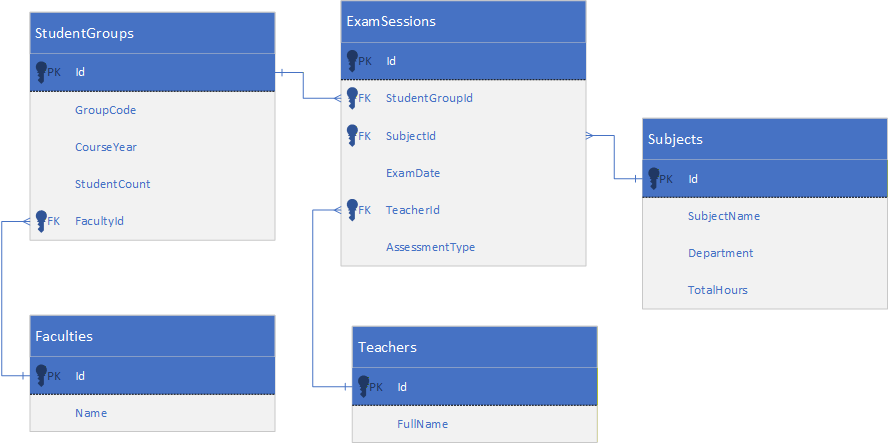
\includegraphics[width=0.92\textwidth]{image.png}
\caption{ER-диаграмма варианта 7}
\label{fig:er}
\end{figure}

\section{Задание 1.2. Создание и заполнение таблиц}
\subsection{Постановка}
По схеме задания~1.1 подготовить DDL с типами, ключами и декларативными ограничениями. Заполнить стержневые сущности не менее чем десятью строками, ассоциативную~--- не менее чем пятнадцатью. Снять SQL-дамп базы.

\subsection{DDL}
Имена столбцов записаны в PascalCase, как в выданной схеме варианта. Первичные ключи~--- \texttt{UUID}, значение по умолчанию даёт \texttt{gen\_random\_uuid()}. Проверки не дают завести курс вне диапазона 1--6, отрицательную численность, нулевой объём дисциплины и произвольную строку вместо формы контроля. Внешние ключи обновляются и удаляются каскадно. Уникальность тройки группа--дисциплина--дата задана отдельным ограничением: суррогатный ключ повторный экзамен не запрещает. Индексы по обоим внешним ключам ускоряют соединение.

\lstinputlisting[language=SQL]{sql/01_schema.sql}

\subsection{Данные}
Загружены 12 групп, 13 дисциплин и 22 экзамена. Экзамен вставляется не по \texttt{UUID}, а соединением с группами и дисциплинами по коду и названию, поэтому скрипт не зависит от сгенерированных ключей. Дисциплина <<Философия>> загружена без экзамена: по ней строится выборка нераспределённых дисциплин и последующее удаление. Полный скрипт вставки:

\lstinputlisting[language=SQL]{sql/02_data.sql}

После загрузки: \texttt{StudentGroups}~--- 12 строк, \texttt{Subjects}~--- 13, \texttt{ExamSessions}~--- 22.

\section{Задание 1.3. Операторы манипулирования}
\subsection{Постановка}
Подготовить четыре осмысленные выборки и по два запроса на вставку, изменение и удаление. В запросах должны встретиться соединение, обобщённое табличное выражение, оконная функция, агрегирование, группировка, вложенный и коррелированный подзапросы.

\subsection{Выборка 1. Нагрузка преподавателя}
Зимняя сессия считается через CTE. К экзамену присоединяется численность группы по \texttt{StudentGroupId}, преподаватели группируются, в выборку попадают те, у кого не меньше двух контролей. Оконная функция считает долю преподавателя во всей сессии, \texttt{ROUND} оставляет три знака.

\begin{lstlisting}[language=SQL]
WITH winter AS (
    SELECT * FROM "ExamSessions"
    WHERE "ExamDate" >= DATE '2026-01-01'
      AND "ExamDate" <  DATE '2026-02-01'
)
SELECT w."TeacherFullName" AS "Преподаватель",
       COUNT(*) AS "Экзаменов",
       COUNT(DISTINCT w."StudentGroupId") AS "Групп",
       SUM(g."StudentCount") AS "Студентов",
       ROUND(100.0 * COUNT(*) / SUM(COUNT(*)) OVER (), 3)
           AS "ДоляСессииПроцент"
FROM winter w
JOIN "StudentGroups" g ON g."Id" = w."StudentGroupId"
GROUP BY w."TeacherFullName"
HAVING COUNT(*) >= 2
ORDER BY "Студентов" DESC;
\end{lstlisting}

\begin{table}[H]
\centering
\caption{Нагрузка преподавателей, январь 2026}
\small
\begin{tabular}{lrrrr}
\toprule
Преподаватель & Экзаменов & Групп & Студентов & Доля, \% \\
\midrule
Кузнецов П.~А. & 3 & 3 & 75 & 18,750 \\
Орлов И.~С. & 3 & 2 & 70 & 18,750 \\
Белова М.~О. & 2 & 2 & 57 & 12,500 \\
Соколова А.~П. & 2 & 2 & 50 & 12,500 \\
Морозова Е.~В. & 2 & 2 & 44 & 12,500 \\
Волков Д.~И. & 2 & 2 & 41 & 12,500 \\
Ершов С.~П. & 2 & 2 & 37 & 12,500 \\
\bottomrule
\end{tabular}
\end{table}
Семь строк дают \(3+3+2+2+2+2+2=16\) экзаменов. Доли сходятся: \(100\cdot16/16=100\).

\subsection{Выборка 2. Дисциплины без сессии}
Левое соединение оставляет дисциплины, которым не нашлось экзамена. Коррелированный подзапрос считает средний объём кафедры.

\begin{lstlisting}[language=SQL]
SELECT s."SubjectName", s."Department", s."TotalHours",
       (SELECT ROUND(AVG(s2."TotalHours"), 3) FROM "Subjects" s2
        WHERE s2."Department" = s."Department") AS "СредниеЧасыКафедры"
FROM "Subjects" s
LEFT JOIN "ExamSessions" e ON e."SubjectId" = s."Id"
WHERE e."SubjectId" IS NULL;
\end{lstlisting}

Результат~--- одна строка: Философия, кафедра гуманитарных наук, 72 часа. Среднее по кафедре тоже 72, дисциплина на кафедре единственная.

\subsection{Выборка 3. Рейтинг групп}
CTE считает число контролей по \texttt{StudentGroupId}. \texttt{ROW\_NUMBER() OVER (PARTITION BY "Faculty")} расставляет места отдельно внутри факультета. Первые места внутри факультета: ЭК-21 (2 контроля), ИВТ-21 (3), ПМ-21 (3), МТ-21 (1). Всего 12 строк, по одной на группу: левое соединение сохраняет группы без экзаменов.
\begin{lstlisting}[language=SQL]
WITH load AS (
    SELECT g."Faculty", g."GroupCode", g."CourseYear",
           COUNT(e."ExamDate") AS "ЧислоКонтролей",
           ROUND(COUNT(e."ExamDate")::numeric
               / NULLIF(g."StudentCount", 0), 3) AS "КонтролейНаСтудента"
    FROM "StudentGroups" g
    LEFT JOIN "ExamSessions" e ON e."StudentGroupId" = g."Id"
    GROUP BY g."Faculty", g."GroupCode", g."CourseYear", g."StudentCount"
)
SELECT "Faculty" AS "Факультет", "GroupCode" AS "Группа",
       "CourseYear" AS "Курс", "ЧислоКонтролей", "КонтролейНаСтудента",
       ROW_NUMBER() OVER (
           PARTITION BY "Faculty"
           ORDER BY "ЧислоКонтролей" DESC, "GroupCode"
       ) AS "МестоНаФакультете"
FROM load
ORDER BY "Факультет", "МестоНаФакультете";
\end{lstlisting}

\begin{table}[H]
\centering
\caption{Вывод выборки 3, 12 строк}
\footnotesize
\begin{tabular}{p{0.36\textwidth}lrrrr}
\toprule
Факультет & Группа & Курс & Контролей & На студента & Место \\
\midrule
Инженерно-экономический институт & ЭК-21 & 4 & 2 & 0,067 & 1 \\
Инженерно-экономический институт & ЭК-22 & 3 & 1 & 0,037 & 2 \\
Институт компьютерных наук & ИВТ-21 & 4 & 3 & 0,125 & 1 \\
Институт компьютерных наук & ИВТ-22 & 3 & 3 & 0,115 & 2 \\
Институт компьютерных наук & ИВТ-23 & 2 & 3 & 0,107 & 3 \\
Институт компьютерных наук & ПИ-21 & 4 & 2 & 0,091 & 4 \\
Институт компьютерных наук & ИБ-23 & 2 & 1 & 0,043 & 5 \\
Институт компьютерных наук & ПИ-22 & 3 & 1 & 0,040 & 6 \\
Институт прикладной математики & ПМ-21 & 4 & 3 & 0,150 & 1 \\
Институт прикладной математики & ПМ-22 & 3 & 1 & 0,048 & 2 \\
Механико-технологический институт & МТ-21 & 4 & 1 & 0,056 & 1 \\
Механико-технологический институт & МТ-22 & 3 & 1 & 0,053 & 2 \\
\bottomrule
\end{tabular}
\end{table}

\subsection{Выборка 4. Ближайший контроль}
Коррелированный \texttt{LATERAL} берёт для группы один экзамен с минимальной датой строго позже 15 января 2026 и подставляет название дисциплины по \texttt{SubjectId}.

\begin{lstlisting}[language=SQL]
SELECT g."GroupCode" AS "Группа",
       nxt."SubjectName" AS "БлижайшаяДисциплина",
       nxt."ExamDate" AS "Дата",
       nxt."TeacherFullName" AS "Преподаватель",
       nxt."AssessmentType" AS "Форма"
FROM "StudentGroups" g
JOIN LATERAL (
    SELECT s."SubjectName", e."ExamDate",
           e."TeacherFullName", e."AssessmentType"
    FROM "ExamSessions" e
    JOIN "Subjects" s ON s."Id" = e."SubjectId"
    WHERE e."StudentGroupId" = g."Id"
      AND e."ExamDate" > DATE '2026-01-15'
    ORDER BY e."ExamDate"
    LIMIT 1
) nxt ON TRUE
ORDER BY nxt."ExamDate", g."GroupCode";
\end{lstlisting}

\begin{table}[H]
\centering
\caption{Вывод выборки 4, 11 строк}
\footnotesize
\begin{tabular}{llp{0.32\textwidth}lp{0.22\textwidth}}
\toprule
Группа & Дата & Дисциплина & Форма & Преподаватель \\
\midrule
ПИ-21 & 16.01 & Базы данных & Экзамен & Орлов И.~С. \\
ИВТ-22 & 18.01 & Компьютерные сети & Экзамен & Орлов И.~С. \\
ИВТ-21 & 19.01 & Операционные системы & Экзамен & Кузнецов П.~А. \\
ПИ-22 & 21.01 & Операционные системы & Диф. зачёт & Кузнецов П.~А. \\
ЭК-21 & 22.01 & Экономика предприятия & Экзамен & Белова М.~О. \\
ПМ-21 & 26.01 & Алгоритмы и структуры данных & Экзамен & Морозова Е.~В. \\
ЭК-22 & 27.01 & Бухгалтерский учёт & Диф. зачёт & Белова М.~О. \\
МТ-21 & 29.01 & Технология машиностроения & Экзамен & Ершов С.~П. \\
МТ-22 & 30.01 & Технология машиностроения & Экзамен & Ершов С.~П. \\
ИВТ-23 & 05.06 & Программирование & Диф. зачёт & Морозова Е.~В. \\
ИБ-23 & 12.06 & Информационная безопасность & Экзамен & Новикова О.~Д. \\
\bottomrule
\end{tabular}
\end{table}




Одиннадцать строк. ПМ-22 в результат не попадает: её экзамен по дискретной математике стоит ровно 15 января, а условие строгое.

\subsection{Изменение 1. Перевод четвёртого курса}
Группы 4 курса института компьютерных наук переводятся на следующий курс. Численность уменьшается на двух отчисленных и не опускается ниже нуля.

\begin{lstlisting}[language=SQL]
UPDATE "StudentGroups"
SET "CourseYear"   = "CourseYear" + 1,
    "StudentCount" = GREATEST("StudentCount" - 2, 0)
WHERE "CourseYear" = 4
  AND "Faculty" = 'Институт компьютерных наук'
RETURNING "GroupCode", "CourseYear", "StudentCount";
\end{lstlisting}

До изменения условию отвечали ИВТ-21 (4 курс, 24) и ПИ-21 (4 курс, 22). Вывод оператора:

\begin{lstlisting}
UPDATE 2
 GroupCode | CourseYear | StudentCount
-----------+------------+--------------
 ИВТ-21    |          5 |           22
 ПИ-21     |          5 |           20
\end{lstlisting}

Повторный отбор групп института оставляет остальные четыре строки прежними: ИВТ-22 (3 курс, 26), ПИ-22 (3 курс, 25), ИБ-23 (2 курс, 23), ИВТ-23 (2 курс, 28).

\subsection{Изменение 2. Дифференцированный зачёт}
Зачёты Соколовой по кафедре вычислительных систем становятся дифференцированными.

\begin{lstlisting}[language=SQL]
UPDATE "ExamSessions" e
SET "AssessmentType" = 'Дифференцированный зачёт'
FROM "Subjects" s
WHERE e."SubjectId" = s."Id"
  AND s."Department" = 'Кафедра вычислительных систем'
  AND e."TeacherFullName" = 'Соколова Анна Петровна'
  AND e."AssessmentType" = 'Зачёт'
RETURNING s."SubjectName", e."ExamDate", e."AssessmentType";
\end{lstlisting}

До изменения условию отвечала одна строка: ИВТ-23, базы данных, 10 июня 2026, зачёт. Вывод оператора:

\begin{lstlisting}
UPDATE 1
 SubjectName |  ExamDate  |      AssessmentType
-------------+------------+--------------------------
 Базы данных | 2026-06-10 | Дифференцированный зачёт
\end{lstlisting}

Январские экзамены Соколовой не затронуты: у ИВТ-21 (12 января) и ИВТ-22 (14 января) форма <<Экзамен>>, а не <<Зачёт>>.
\subsection{Вставка 1. Новая дисциплина и зачёт}
В перечень добавляется дисциплина <<Криптографические методы>> и первый зачёт по ней для группы ИБ-23.

\begin{lstlisting}[language=SQL]
INSERT INTO "Subjects" ("SubjectName", "Department", "TotalHours")
VALUES ('Криптографические методы', 'Кафедра защиты информации', 72);

INSERT INTO "ExamSessions"
    ("StudentGroupId", "SubjectId", "ExamDate",
     "TeacherFullName", "AssessmentType")
SELECT g."Id", s."Id", DATE '2026-06-18',
       'Новикова Ольга Дмитриевна', 'Зачёт'
FROM "StudentGroups" g
JOIN "Subjects" s ON s."SubjectName" = 'Криптографические методы'
WHERE g."GroupCode" = 'ИБ-23';
\end{lstlisting}

Оба оператора вернули \texttt{INSERT 0 1}. Проверочная выборка по названию дисциплины дала одну строку:

\begin{lstlisting}
 GroupCode | SubjectName              | Department
-----------+--------------------------+---------------------------
 ИБ-23     | Криптографические методы | Кафедра защиты информации

 TotalHours | ExamDate   | TeacherFullName           | AssessmentType
------------+------------+---------------------------+----------------
         72 | 2026-06-18 | Новикова Ольга Дмитриевна | Зачёт
\end{lstlisting}

\subsection{Вставка 2. Пересдача баз данных}
Январский экзамен по базам данных назначается повторно через 30 дней. Дата берётся из уже существующей строки.

\begin{lstlisting}[language=SQL]
INSERT INTO "ExamSessions"
    ("StudentGroupId", "SubjectId", "ExamDate",
     "TeacherFullName", "AssessmentType")
SELECT e."StudentGroupId", e."SubjectId", e."ExamDate" + 30,
       e."TeacherFullName", 'Экзамен'
FROM "ExamSessions" e
JOIN "Subjects" s ON s."Id" = e."SubjectId"
WHERE s."SubjectName" = 'Базы данных'
  AND e."AssessmentType" = 'Экзамен'
  AND e."ExamDate" < DATE '2026-02-01';
\end{lstlisting}

До вставки по базам данных было четыре строки: три январских экзамена и июньский дифференцированный зачёт ИВТ-23. Оператор вернул \texttt{INSERT 0 3}. Повторный отбор дал семь строк:

\begin{lstlisting}
 GroupCode | ExamDate   | TeacherFullName        | AssessmentType
-----------+------------+------------------------+----------------
 ИВТ-21    | 2026-01-12 | Соколова Анна Петровна | Экзамен
 ИВТ-21    | 2026-02-11 | Соколова Анна Петровна | Экзамен
 ИВТ-22    | 2026-01-14 | Соколова Анна Петровна | Экзамен
 ИВТ-22    | 2026-02-13 | Соколова Анна Петровна | Экзамен
 ИВТ-23    | 2026-06-10 | Соколова Анна Петровна | Диф. зачёт
 ПИ-21     | 2026-01-16 | Орлов Игорь Сергеевич  | Экзамен
 ПИ-21     | 2026-02-15 | Орлов Игорь Сергеевич  | Экзамен
\end{lstlisting}

Июньский зачёт ИВТ-23 не продублирован: фильтр требует форму <<Экзамен>> и дату раньше 1 февраля.

\subsection{Удаление 1. Снятие пересдачи}
Пересдача снимается, если по той же паре группа--дисциплина уже есть более ранний экзамен. Проверка идёт коррелированным \texttt{EXISTS}.

\begin{lstlisting}[language=SQL]
DELETE FROM "ExamSessions" e
USING "Subjects" s
WHERE e."SubjectId" = s."Id"
  AND s."SubjectName" = 'Базы данных'
  AND e."ExamDate" >= DATE '2026-02-01'
  AND EXISTS (
      SELECT 1
      FROM "ExamSessions" earlier
      WHERE earlier."StudentGroupId" = e."StudentGroupId"
        AND earlier."SubjectId" = e."SubjectId"
        AND earlier."ExamDate" < e."ExamDate"
  );
\end{lstlisting}

Оператор вернул \texttt{DELETE 3}: сняты 11, 13 и 15 февраля. Повторный отбор снова даёт четыре исходные строки:

\begin{lstlisting}
 GroupCode | ExamDate   | TeacherFullName        | AssessmentType
-----------+------------+------------------------+--------------------------
 ИВТ-21    | 2026-01-12 | Соколова Анна Петровна | Экзамен
 ИВТ-22    | 2026-01-14 | Соколова Анна Петровна | Экзамен
 ИВТ-23    | 2026-06-10 | Соколова Анна Петровна | Дифференцированный зачёт
 ПИ-21     | 2026-01-16 | Орлов Игорь Сергеевич  | Экзамен
\end{lstlisting}

\subsection{Удаление 2. Дисциплины вне сессии}
Удаляются дисциплины, которым не соответствует ни одна строка экзамена.

\begin{lstlisting}[language=SQL]
DELETE FROM "Subjects" s
WHERE NOT EXISTS (
    SELECT 1 FROM "ExamSessions" e WHERE e."SubjectId" = s."Id"
)
RETURNING s."SubjectName", s."Department";
\end{lstlisting}

До удаления таким был единственный предмет. Вывод оператора:

\begin{lstlisting}
DELETE 1
 SubjectName | Department
-------------+---------------------------
 Философия   | Кафедра гуманитарных наук
\end{lstlisting}

Криптографические методы сохранены: на них ссылается зачёт ИБ-23. После удаления в таблице 13 дисциплин, и каждая встречается в сессии.

\section{Задание 1.4. Контроль целостности}
\subsection{Постановка}
Проверить потерянное обновление, грязное чтение, неповторяющееся чтение, фантом и аномалию сериализации на уровнях SQL/92. Написать два триггера: один поправляет данные, второй откатывает транзакцию.

Опыты идут по \texttt{StudentGroups.StudentCount}. Исходно ИВТ-21~--- 24, ИВТ-22~--- 26. В PostgreSQL READ UNCOMMITTED работает как READ COMMITTED, поэтому грязного чтения нет ни на одном уровне.

\subsection{Сводка}
\begin{table}[H]
\centering
\caption{Аномалии в PostgreSQL 16}
\small
\begin{tabular}{lccc}
\toprule
Аномалия & RC (и RU) & RR & Serializable \\
\midrule
Потерянное обновление & нет & нет & нет \\
Грязное чтение & нет & нет & нет \\
Неповторяющееся чтение & да & нет & нет \\
Фантом & да & нет & нет \\
Сериализация & --- & да & откат \\
\bottomrule
\end{tabular}
\end{table}

\subsection{Потерянное обновление}
Проверяется инкрементами, не присваиванием константы. A прибавляет 1, B прибавляет 10. Без аномалии итог равен \(24+1+10=35\).

\begin{table}[H]
\centering
\caption{Ход сеансов, READ COMMITTED}
\small
\begin{tabular}{p{0.46\textwidth}p{0.46\textwidth}}
\toprule
Транзакция A & Транзакция B \\
\midrule
BEGIN, READ COMMITTED & \\
 & BEGIN, READ COMMITTED \\
UPDATE +1, видит 25 & \\
 & UPDATE +10, ждёт блокировку \\
COMMIT & \\
 & дожидается, пишет 35, COMMIT \\
\bottomrule
\end{tabular}
\end{table}
Итог~--- 35, оба инкремента живы. На REPEATABLE READ строка блокируется так же.

\subsection{Грязное и неповторяющееся чтение}
A прибавляет 100 и не фиксирует транзакцию. B читает ИВТ-21 и получает 24, а не 124. После отката A чужое значение так и не стало видимым.

Неповторяющееся чтение: A читает 24, B пишет 40 и фиксируется, A читает снова. READ COMMITTED возвращает 40, REPEATABLE READ возвращает 24.

\subsection{Фантом}
A дважды считает группы первого курса. Между подсчётами B вставляет PHANTOM-99 с курсом 1. READ COMMITTED меняет счётчик с 0 на 1, REPEATABLE READ оба раза даёт 0.

\subsection{Сериализация}
A пишет в ИВТ-21 значение ИВТ-22. B пишет в ИВТ-22 значение ИВТ-21 из своего снимка. Последовательно A, затем B, даёт (26, 26). Параллельно на REPEATABLE READ получается (26, 24): такого состояния нет ни в одном последовательном порядке. На SERIALIZABLE вторая транзакция получает ошибку
\texttt{could not serialize access} и откатывается, остаётся (26, 26).

\subsection{Триггеры}
\texttt{trg\_limit\_student\_drop} срабатывает до обновления численности. Падение больше чем на 5 человек срезается, транзакция остаётся жива. МТ-22 имела 19 человек, запрос ставил 1, в таблице осталось 14.

\texttt{trg\_check\_exam\_date} запрещает экзамен в выходной и второй контроль группы в тот же день. 20 июня 2026~--- суббота, вставка экзамена МТ-21 отклонена. Вставка компьютерных сетей для ИВТ-21 на 12 января отклонена: в этот день у группы уже стоят базы данных. Оба отказа откатывают оператор.

\subsection{Выводы по заданию 1.4}
В PostgreSQL READ UNCOMMITTED работает как READ COMMITTED, поэтому грязного чтения нет ни на одном уровне. Потерянное обновление проверяется инкрементами, а не присваиванием константы. Аномалия сериализации получается перекрёстным обновлением двух строк. На SERIALIZABLE вторая транзакция откатывается, на REPEATABLE READ аномалия остаётся.

\section{Задание 2.1. Управление доступом}
\subsection{Постановка}
Создать пользователя \texttt{test}, раздать разные права на разные таблицы, сделать однотабличное и многотабличное представления, разрешить вставку в многотабличное представление и завести роль с UPDATE на отдельные столбцы. Права показать командой \texttt{\textbackslash dp}.

\subsection{Права и представления}
\texttt{test} получает LOGIN, \texttt{CONNECT} на базу и \texttt{USAGE} на схему. На \texttt{StudentGroups} выданы SELECT, INSERT и UPDATE. На \texttt{Subjects}~--- чтение всех столбцов и UPDATE только \texttt{TotalHours}. На \texttt{ExamSessions}~--- только SELECT.

\texttt{v\_exam\_card}~--- представление экзаменов без зачётов. Оно соединяет \texttt{ExamSessions} с группой и дисциплиной, чтобы в карточке был код группы и название, а не суррогатные ключи. \texttt{test} читает из него 16 строк. \texttt{v\_group\_load} соединяет группу с числом контролей. Вставку обрабатывает триггер \texttt{INSTEAD OF INSERT}: пишется строка группы, вычисляемый столбец игнорируется, \texttt{Id} группа получает сама. От имени \texttt{test} так создана группа ТЕСТ-01, 1 курс, 17 человек.

Роль \texttt{exam\_editor} выдана пользователю \texttt{test}. Через представление \texttt{v\_group\_headcount} она меняет только \texttt{StudentCount} и только у института компьютерных наук: у представления стоят \texttt{security\_barrier} и \texttt{check\_option}. Материализованное \texttt{mv\_faculty\_stats} хранит готовый агрегат по факультетам и не пересчитывает соединение на каждый просмотр.

\subsection{Проверка от имени test}
SELECT по группе проходит. UPDATE часов баз данных проходит: 144 становится 150. UPDATE кафедры отклоняется, \texttt{permission denied for table Subjects}. INSERT в \texttt{ExamSessions} отклоняется так же. UPDATE численности ИВТ-23 через представление роли проходит, значение становится 29. Такой же UPDATE для МТ-21 меняет 0 строк: чужой факультет не проходит \texttt{CHECK OPTION}.

Команда \texttt{\textbackslash dp exam.*} показывает флаги: \texttt{r}~--- чтение, \texttt{a}~--- вставка, \texttt{w}~--- обновление, \texttt{d}~--- удаление, \texttt{D}~--- очистка, \texttt{x}~--- ссылка, \texttt{t}~--- триггер. У \texttt{ExamSessions} для \texttt{test} стоит \texttt{r}, у \texttt{StudentGroups}~--- \texttt{arw}. В столбцовых привилегиях \texttt{TotalHours} имеет \texttt{rw}, остальные столбцы \texttt{Subjects}~--- \texttt{r}.

\subsection{Выводы по заданию 2.1}
Столбцовые права в выводе \texttt{\textbackslash dp} выводятся отдельной колонкой, рядом с табличными флагами их легко пропустить. \texttt{CHECK OPTION} не заменяет привилегию: МТ-21 не обновилась, потому что строка не видна представлению, а не потому что нет права. Вставка в соединение без \texttt{INSTEAD OF} невозможна: строку нельзя однозначно разложить по таблицам. На Windows перед \texttt{\textbackslash dp} в \texttt{psql} нужна команда \texttt{\textbackslash ! chcp 1251}, иначе кириллица в именах распадается.

\section{Задание 2.2. Функции и PL/pgSQL}
\subsection{Постановка}
Написать три-четыре функции, которые упрощают работу с данными. В коде должны быть переменные, ветвления, циклы, курсор и обработка исключений. Отдельно показать, чем функция удобнее представления.

\subsection{Назначение экзамена}
\texttt{exam.schedule\_exam} проверяет, что группа и дисциплина существуют, и берёт их \texttt{Id}. Форма контроля должна входить в допустимый список. Повторная вставка той же тройки группа--дисциплина--дата перехватывается секцией \texttt{EXCEPTION} по \texttt{unique\_violation} и заменяется понятным текстом. Уникальность держит отдельное ограничение, а не первичный ключ. Успешный вызов поставил зачёт МТ-21 по базам данных на 22 июня 2026. Повторный вызов вернул <<контроль уже назначен>>. Код~--- \texttt{sql/07\_functions.sql}.

\subsection{Ведомость преподавателя}
\texttt{exam.teacher\_sheet} открывает курсор по экзаменам преподавателя, в цикле \texttt{LOOP} забирает строку и ветвлением \texttt{IF/ELSIF} переводит форму контроля в короткий код. Для Соколовой функция вернула три строки:

\begin{lstlisting}
1. 2026-01-12  ИВТ-21  ЭКЗ  Базы данных
2. 2026-01-14  ИВТ-22  ЭКЗ  Базы данных
3. 2026-06-10  ИВТ-23  ЗАЧ  Базы данных
\end{lstlisting}

\subsection{Перенос сессии группы}
\texttt{exam.postpone\_group} в цикле \texttt{FOR} по выборке сдвигает даты группы на заданное число дней и внутренним циклом перепрыгивает субботу и воскресенье. Неположительный сдвиг отвергается исключением. Для МТ-22 сдвиг на 3 дня перенёс экзамен с 30 января на 2 февраля: 1 февраля 2026~--- воскресенье, функция ушла на понедельник. Возвращено число сдвинутых строк, оно равно 1.

\subsection{Сводка факультета}
\texttt{exam.faculty\_report} возвращает таблицу из четырёх столбцов. Переменные держат число групп, студентов и контролей, ветвление собирает комментарий. Для института компьютерных наук: 6 групп, 148 студентов, 13 контролей, <<нагрузка выше двух контролей на группу>>. Неизвестный факультет поднимает исключение, а не пустую таблицу.

\subsection{Функция против представления}
Представление~--- сохранённый запрос без параметров и без права прервать операцию. Функция принимает факультет и преподавателя аргументами, проверяет вход до изменения данных и возвращает либо таблицу, либо текст ведомости. Отказ с текстом на русском сообщает причину, а не сырой код нарушения ключа. Карточка экзамена из задания 2.1 остаётся представлением: ей не нужны параметры и проверка входа.

\subsection{Выводы по заданию 2.2}
Ведомость можно собрать одним запросом. Курсор оставлен, чтобы показать построчную обработку: \texttt{FETCH}, \texttt{EXIT WHEN NOT FOUND} и ветвление по форме контроля. Сдвиг дат идёт циклом, потому что правило выходного дня в \texttt{WHILE} записывается прямо. Секция \texttt{EXCEPTION} ловит конкретный \texttt{SQLSTATE}. Перехват \texttt{OTHERS} скрыл бы и сбой схемы, и настоящий отказ ограничения.

\section*{Заключение}
\addcontentsline{toc}{section}{Заключение}
Собрана база учёта сессии из двух стержневых сущностей и одной ассоциативной. Идентификаторы сущностей~--- \texttt{UUID}, связи идут по ним, а код группы и название дисциплины остаются уникальными естественными ключами. База заполнена и проверена запросами с соединением, CTE, окном и коррелированным подзапросом. В PostgreSQL грязного чтения нет: READ UNCOMMITTED совпадает с READ COMMITTED. Потерянное обновление закрыто блокировкой строки. Аномалия сериализации возникает на REPEATABLE READ и откатывается на SERIALIZABLE. Триггеры проверяют условия, которые не выражаются столбцовым \texttt{CHECK}. Роли и представления отрезают пользователю \texttt{test} чужие столбцы и чужие таблицы. Функции принимают параметры, проверяют вход и возвращают текст ошибки.

\end{document}





